\documentclass[submit]{harvardml}

\course{CS181-S21}
\assignment{Assignment \#1}
\duedate{7:59pm ET, February 4, 2021}

\usepackage[OT1]{fontenc}
\usepackage[colorlinks,citecolor=blue,urlcolor=blue]{hyperref}
\usepackage[pdftex]{graphicx}
\usepackage{graphicx}
\usepackage{caption}
\usepackage{fullpage}
\usepackage{soul}
\usepackage{amsmath}
\usepackage{amssymb}
\usepackage{color}
\usepackage{todonotes}
\usepackage{listings}
\usepackage{common}
\usepackage{framed}
\usepackage{physics}

\usepackage[mmddyyyy,hhmmss]{datetime}

\definecolor{verbgray}{gray}{0.9}

\lstnewenvironment{csv}{
  \lstset{backgroundcolor=\color{verbgray},
  frame=single,
  framerule=0pt,
  basicstyle=\ttfamily,
  columns=fullflexible}}{}


\begin{document}
\begin{center}
{\Large Homework 1: Regression}\\
\end{center}

\subsection*{Introduction}
This homework is on different forms of linear regression and focuses
on loss functions, optimizers, and regularization. Linear regression
will be one of the few models that we see that has an analytical
solution.  These problems focus on deriving these solutions and
exploring their properties.

If you find that you are having trouble with the first couple
problems, we recommend going over the fundamentals of linear algebra
and matrix calculus (see links on website).  The relevant parts of the
\href{https://github.com/harvard-ml-courses/cs181-textbook/blob/master/Textbook.pdf}{cs181-textbook notes are Sections 2.1 - 2.7}.  We strongly recommend
reading the textbook before beginning the homework.

    We also encourage you to first read the \href{http://users.isr.ist.utl.pt/~wurmd/Livros/school/Bishop\%20-\%20Pattern\%20Recognition\%20And\%20Machine\%20Learning\%20-\%20Springer\%20\%202006.pdf}{Bishop textbook}, particularly:
Section 2.3 (Properties of Gaussian Distributions), Section 3.1
(Linear Basis Regression), and Section 3.3 (Bayesian Linear
Regression). (Note that our notation is slightly different but the
underlying mathematics remains the same!).

\textbf{Please type your solutions after the corresponding problems using this
\LaTeX\ template, and start each problem on a new page.} You may find
the following introductory resources on \LaTeX\ useful:
\href{http://www.mjdenny.com/workshops/LaTeX_Intro.pdf}{\LaTeX\ Basics}
and \href{https://www.overleaf.com/learn/latex/Free_online_introduction_to_LaTeX_(part_1)}{\LaTeX\ tutorial with exercises in Overleaf}

Homeworks will be submitted through Gradescope. You will be added to
the course Gradescope once you join the course Canvas page. If you
haven't received an invitation, contact the course staff through Ed.

\textbf{Please submit the writeup PDF to the Gradescope assignment
  `HW1'.} Remember to assign pages for each question.

\textbf{Please submit your \LaTeX file and code files to the
  Gradescope assignment `HW1 - Supplemental'.} Your files should be
named in the same way as we provide them in the repository,
e.g. \texttt{T1\_P1.py}, etc.


%%%%%%%%%%%%%%%%%%%%%%%%%%%%%%%%%%%%%%%%%%%%%
% Problem 1
%%%%%%%%%%%%%%%%%%%%%%%%%%%%%%%%%%%%%%%%%%%%%


\begin{problem}[Optimizing a Kernel, 15pts]

Kernel-based regression techniques are similar to nearest-neighbor
regressors: rather than fit a parametric model, they predict values
for new data points by interpolating values from existing points in
the training set.  In this problem, we will consider a kernel-based
regressor of the form:
\begin{equation*}
  f(x^*) = \frac{ \sum_{n} K(x_n,x^*) y_n  }{ \sum_{n} K(x_n,x^*) }
\end{equation*}
where $(x_n,y_n)$ are the training data points, and $K(x,x')$ is a
kernel function that defines the similarity between two inputs $x$ and
$x'$. Assume that each $x_i$ is represented as a column vector, i.e. a
$D$ by 1 vector where $D$ is the number of features for each data
point. A popular choice of kernel is a function that decays as the
distance between the two points increases, such as
\begin{equation*}
  K(x,x') = \exp(-||x-x'||^2_2) = \exp(-(x-x')^T (x-x') )
\end{equation*}
However, the squared Euclidean distance $||x-x'||^2_2$ may not always
be the right choice.  In this problem, we will consider optimizing
over squared Mahalanobis distances
\begin{equation*}
  K(x,x') = \exp(-(x-x')^T W (x-x') )
  \label{eqn:distance}
\end{equation*}
where $W$ is a symmetric $D$ by $D$ matrix.  Intuitively, introducing
the weight matrix $W$ allows for different dimensions to matter
differently when defining similarity.

\begin{enumerate}

\item Let $\{(x_n,y_n)\}_{n=1}^N$ be our training data set.  Suppose
  we are interested in minimizing the residual sum of squares.  Write down this
  loss over the training data $\mcL(W)$ as a function of $W$.

  Important: When computing the prediction $f(x_i)$ for a point $x_i$
  in the training set, carefully consider for which points $x'$ you should be including
  the term $K(x_i,x')$ in the sum.

\item In the following, let us assume that $D = 2$.  That means that
  $W$ has three parameters: $W_{11}$, $W_{22}$, and $W_{12} = W_{21}$.
  Expand the formula for the loss function to be a function of these
  three parameters.

 \item Derive the gradients of the loss function with respect to each of the parameters of $W$ for the $D=2$ case. (This will look a bit messy!)



\end{enumerate}
\end{problem}


\newpage

\begin{framed}
\noindent\textbf{Problem 1} (cont.)\\
\begin{enumerate}
\setcounter{enumi}{3}
\item Consider the following data set:
\begin{csv}
x1 , x2 , y
  0 , 0 , 0
  0 , .5 , 0
  0 , 1 , 0
  .5 , 0 , .5
  .5 , .5 , .5
  .5 , 1 , .5
  1 , 0 , 1
  1 , .5 , 1
  1 , 1 , 1
\end{csv}
And the following kernels:
\begin{equation*}
W_1 = \alpha \begin{bmatrix}
  1 & 0 \\
  0 & 1
\end{bmatrix}
\qquad
W_2 = \alpha \begin{bmatrix}
  0.1 & 0 \\
  0 & 1
\end{bmatrix}
\qquad
W_3 = \alpha \begin{bmatrix}
  1 & 0 \\
  0 & 0.1
\end{bmatrix}
\end{equation*}
with $\alpha = 10$. Write some Python code to compute the loss with
respect to each kernel for the dataset provided above. Which kernel
does best?  Why?  How does the choice of $\alpha$ affect the loss?

For this problem, you can use our staff \textbf{script to compare your code to a set of staff-written test cases.} This requires, however, that you use the structure of the starter code provided in \texttt{T1\_P1.py}. More specific instructions can be found at the top of the file \texttt{T1\_P1\_Testcases.py}. You may run the test cases in the command-line using \texttt{python T1\_P1\_TestCases.py}.
\textbf{Note that our set of test cases is not comprehensive: just because you pass does not mean your solution is correct! We strongly encourage you to write your own test cases and read more about ours in the comments of the Python script.}

\item Bonus:  Code up a gradient descent to
  optimize the kernel for the data set above.  Start your gradient
  descent from $W_1$.  Report on what you find.\\
  Gradient descent is discussed in Section 3.4 of the cs181-textbook notes and Section 5.2.4 of Bishop, and will be covered later in the course!

\end{enumerate}

\end{framed}

\newpage

Problem 1 Solution:
\begin{enumerate}
    \item If our loss is to be the residual sum of squares, then we can generally write it as $\mcL(W)=\sum_{n=1}^N (y_n - \hat{y}_n)^2$. We also know that $\hat{y}_n = f(x_n) = \frac{\sum_{i \neq n} K(x_i, x_n)y_i}{\sum_{i \neq n} K(x_i, x_n)}$. Note that the $i$ in that last expression is meant to denote all $i$ from 1 to $N$ , inclusive, excluding $n$, the subscript of the input $x_n$. This is because if we do not exclude that particular index and thus compute the kernel on the input data point to itself, all the weight will be placed on that data point at the exclusion of the other points (since you are closest to yourself), which will lead to perfect predictions. This ignores the predictive power of the rest of the dataset and is overfitting to our current dataset, which will lead to poor test performance. You can imagine a scenario illustrating this if we imagine a dataset with many points clustered around a veritable line, except for one outlier. When we go to find the predicted $\hat{y}_n$ for that $x_n$, it would make much more sense to consider the rest of the dataset rather than predict based on the data we have on that particular input. Therefore, we can substitute this in, along with the expression for Mahalanobis distance to get:

    $$\mcL(W)=\sum_{n=1}^N (y_n - \frac{\sum_{i \neq n} \exp(-(x_i-x_n)^TW(x_i-x_n))y_i}{\sum_{i \neq n} \exp(-(x_i-x_n)^TW(x_i-x_n))})^2$$

    \item We will need to break down matrices and vectors into their components to solve this problem. Note that
    \begin{equation*}
        x_n = \begin{bmatrix}
          x_{n1} \\
          x_{n2}
        \end{bmatrix}
        \qquad
        x_i - x_n =
        \begin{bmatrix}
          x_{i1} - x_{n1} \\
          x_{i2} - x_{n2}
        \end{bmatrix}
    \end{equation*}

    which means that $W(x-x^')$ can be written as
    \begin{equation*}
        \begin{bmatrix}
          W_{11} & W_{12} \\
          W_{21} & W_{22}
        \end{bmatrix}
        \begin{bmatrix}
          x_{i1} - x_{n1} \\
          x_{i2} - x_{n2}
        \end{bmatrix} =
        \begin{bmatrix}
          W_{11}(x_{i1} - x_{n1}) + W_{12}(x_{i2} - x_{n2}) \\
          W_{21}(x_{i1} - x_{n1}) + W_{22}(x_{i2} - x_{n2})
        \end{bmatrix}
    \end{equation*}

    and then $-(x-x')^T W (x-x')$ can be written as
    $$W_{11}(x_{i1} - x_{n1})^2 + W_{12}(x_{i1} - x_{n1})(x_{i2} - x_{n2}) +  W_{21}(x_{i1} - x_{n1})(x_{i2} - x_{n2}) + W_{22}(x_{i2} - x_{n2})^2$$
    $$= W_{11}(x_{i1} - x_{n1})^2 + 2W_{12}(x_{i1} - x_{n1})(x{i2} - x_{n2}) + W_{22}(x{i2} - x_{n2})^2$$

    Then we can rewrite the loss function as

    $$\mcL(W)=\sum_{n=1}^N (y_n - \frac{\sum_{i \neq n} \exp(-(W_{11}(x_{i1} - x_{n1})^2 + 2W_{12}(x_{i1} - x_{n1})(x_{i2} - x_{n2}) + W_{22}(x_{i2} - x_{n2})^2))y_i}{\sum_{i \neq n} \exp(-(W_{11}(x_{i1} - x_{n1})^2 + 2W_{12}(x_{i1} - x_{n1})(x_{i2} - x_{n2}) + W_{22}(x{i2} - x_{n2})^2))})^2$$

    \item As a form of shorthand moving forward, let's make the following substitutions for the sake of readability:

    $$J_{n,i} = \exp(-(W_{11}(x_{i1} - x_{n1})^2 + 2W_{12}(x_{i1} - x_{n1})(x_{i2} - x_{n2}) + W_{22}(x_{i2} - x_{n2})^2))$$

    $$v_{ij1} = x_{i1} - x_{n1}$$

    $$v_{ij2} = x_{i2} - x_{n2}$$

    Note the following:

    $$\pdv{J_{n,i}}{W_{11}} = -J_{n,i}(v_{ij1})^2$$

    $$\pdv{J_{n,i}}{W_{11}} = -J_{n,i}(v_{ij2})^2$$

    $$\pdv{J_{n,i}}{W_{12}} = \pdv{J_{n,i}}{W_{21}} = -2J_{n,i}(v_{ij1})(v_{ij2})$$

    Then we have the following, after applying the chain rule, and then the division rule on $\frac{\sum_{i \neq n} J_{n,i}y_i}{\sum_{i \neq n} J_{n,i}}$:

    $$\pdv{}{W_{11}}\mcL(W) = \sum_{n=1}^N -2(y-\frac{\sum_{i \neq n} J_{n,i}y_i}{\sum_{i \neq n} J_{n,i}})(\frac{[\sum_{i \neq n} -J_{n,i}(v_{ij1})^2y_i][\sum_{i \neq n} J_{n,i}] - [\sum_{i \neq n} -J_{n,i}(v_{ij1})^2][\sum_{i \neq n} J_{n,i}y_i ]}{[\sum_{i \neq n} J_{n,i}]^2})$$

    $$\pdv{}{W_{22}}\mcL(W) = \sum_{n=1}^N -2(y-\frac{\sum_{i \neq n} J_{n,i}y_i}{\sum_{i \neq n} J_{n,i}})(\frac{[\sum_{i \neq n} -J_{n,i}(v_{ij2})^2y_i][\sum_{i \neq n} J_{n,i}] - [\sum_{i \neq n} -J_{n,i}(v_{ij2})^2][\sum_{i \neq n} J_{n,i}y_i ]}{[\sum_{i \neq n} J_{n,i}]^2})$$

    $$\pdv{}{W_{12}}\mcL(W) = \pdv{}{W_{21}}\mcL(W) $$
    $$= \sum_{n=1}^N -2(y-\frac{\sum_{i \neq n} J_{n,i}y_i}{\sum_{i \neq n} J_{n,i}})(\frac{[\sum_{i \neq n} -2J_{n,i}(v_{ij1})(v_{ij2})y_i][\sum_{i \neq n} J_{n,i}] - [\sum_{i \neq n} -2J_{n,i}(v_{ij1})(v_{ij2})][\sum_{i \neq n} J_{n,i}y_i ]}{[\sum_{i \neq n} J_{n,i}]^2})$$

    \item For $W_1$, the loss is 0.33821615730087107. For $W_2$, the loss is 2.2263823122858097. For $W_3$, the loss is 0.024847637804324457. Thus, based on which kernel results in predictions with minimal loss, $W_3$ does best. Given that alpha is constant across these kernels, we only consider how $W$ affects this result. Since $W_{12}=W_{21}$ and we only have positive terms for $W_11$ and $W_22$, these two values, respectively, tell us how much to weight the first and second component of the input data vector. $W_3$ working best means that weighting the first component of $x$ 10 times more than the second component is most effective, meaning that the first component of $x$ is more indicative of $y$ than the second component. This can be seen reflected in the data since $y$ is always equal to the first component of $x$, but not always equal to the second component of $x$.

    The choice of alpha is essentially a discount factor. The higher $\alpha$ is, the more we discount points that are farther away from the input when we go to compute the Mahalanobis distance. To see this quantitatively, note that a higher alpha will inflate the terms of $W$, leading us to compute $K$ where we are raising to a larger negative factor, which pushes the value of $K$ down. If we conversely use a lower alpha, the oppositve will occur. The relative ranking of the weights does not change, only their actual values. A higher alpha also serves to exaggerate the difference in how we weight the components of x, and $W_3$'s loss decreasing in the chart below as we increase alpha to put even more weight on that first component compared to the second component is consistent with this idea. Running a few test cases, we observe the following:

    \begin{center}
        \begin{tabular}{ |c|c|c|c| }
         \hline
         Alpha/Loss & $W_1$ Loss & $W_2$ Loss & $W_3$ Loss \\
         \hline
         $\alpha=0.1$ & 1.8094301740585537 & 1.9036901684095073 & 1.7952358038005056\\
         \hline
         $\alpha=1$ & 1.1840178839616164 & 1.9565443053118377 & 1.0593632813080032\\
         \hline
         $\alpha=10$ & 0.33821615730087107 & 2.2263823122858097 & 0.024847637804324457\\
         \hline
         $\alpha=50$ & 0.3055570393147468 & 1.569670854256359 & 3.2243135747543195e-10\\
         \hline
         $\alpha=100$ & 0.3055555555610851 & 1.5016587935799697 & 3.8332638952736116e-20\\
         \hline
        \end{tabular}
    \end{center}

    From this, we can see that decreasing alpha increases the loss and increasing alpha decreases the loss for $W_1$ and $W_3$. For $W_2$, both increasing and decreasing alpha seem to decrease the loss. However, the ranking $\mcL(W_3) < \mcL(W_1) < \mcL(W_2)$ doesn't seem to change given a fixed alpha, for all alpha.
\end{enumerate}

\newpage

%%%%%%%%%%%%%%%%%%%%%%%%%%%%%%%%%%%%%%%%%%%%%
% Problem 2
%%%%%%%%%%%%%%%%%%%%%%%%%%%%%%%%%%%%%%%%%%%%%


\begin{problem}[Kernels and kNN, 10pts]

Now, let us compare the kernel-based approach to an approach based on
nearest-neighbors.  Recall that kNN uses a predictor of the form

  \begin{equation*}
    f(x^*) = \frac{1}{k} \sum_n y_n \mathbb{I}(x_n \texttt{ is one of k-closest to } x^*)
  \end{equation*}

\noindent where $\mathbb{I}$ is an indicator variable. For this problem, you will use the same kernels as Problem 1, and dataset \verb|data/p2.csv|.

For this problem, you can use our staff \textbf{script to compare your code to a set of staff-written test cases.} This requires, however, that you use the structure of the starter code provided in \texttt{T1\_P2.py}. More specific instructions can be found at the top of the file \texttt{T1\_P2\_Testcases.py}. You may run the test cases in the command-line using \texttt{python T1\_P2\_TestCases.py}.
\textbf{Note that our set of test cases is not comprehensive: just because you pass does not mean your solution is correct! We strongly encourage you to write your own test cases and read more about ours in the comments of the Python script.}

\vspace{0.5cm}
\noindent\emph{Make sure to include all required plots in your PDF.}


\begin{enumerate}

\item We will be making 6 plots comparing kernel-based and nearest
  neighbor-based predictors, all using the Mahalanobis distance
  corresponding to $W_1$ from Problem 1. In each plot, you will plot
  the predicted value of $y$, given $x_1$ (horizontal axis) and $x_2$
  (vertical axis), as the color of each point (grayscale
  between $0$ and $1$). Include the $x_1$ and $x_2$ axes, with tick marks spaced every 0.1 units
  for $x_1=0$ to $x_1=1$ and $x_2=0$ to $x_2=1$.

  For the first three plots, use the kernel-based predictor varying
  $\alpha = \{0.1,3,10\}$.  For the next three plots, use the kNN
  predictor with $\alpha = 1$, $k=\{1,5,N-1\}$, where $N$ is the size
  of the data set.

  Print the total least squares loss on the training set for each of
  the 6 plots.

  You may choose to use some starter Python code to create your plots
  provided in \verb|T1_P2.py|.  Please \textbf{write your own
    implementation of kNN} for full credit.  Do not use external
  libraries to find nearest neighbors.

\item Do any of the kernel-based regression plots look like the 1NN?
  The $(N-1)$NN?  Why or why not?

\item Suppose we are given some $W$ for a Mahalanobis distance or
  kernel function.  Then, in general, there exist values of $k$ for which
  kernel-based regression and kNN disagree (i.e., make different predictions)
  on at least one input - for all choices of $\alpha$. Explain why by means of
  an example (i.e., show that for some value $k$ of your choosing,
  no value of $\alpha$ will produce two classifiers that are the same).

\item Why did we not vary $\alpha$ for the kNN approach?

\end{enumerate}

\end{problem}

\newpage

Problem 2 Solution:

\begin{enumerate}
    \item My plots, with losses (also printed to terminal):

    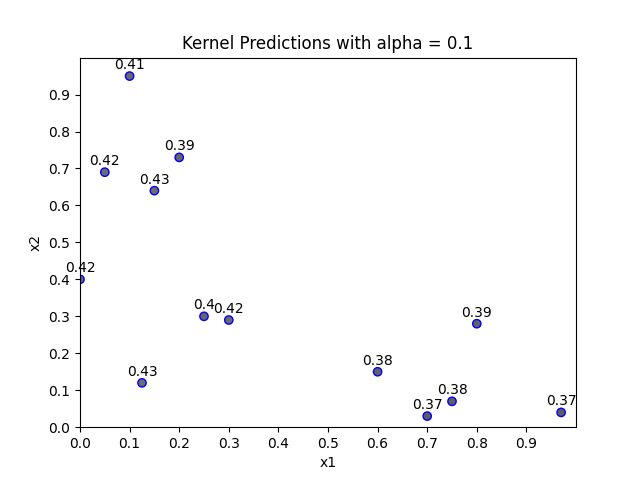
\includegraphics[scale=0.6]{alpha0.1.png}

    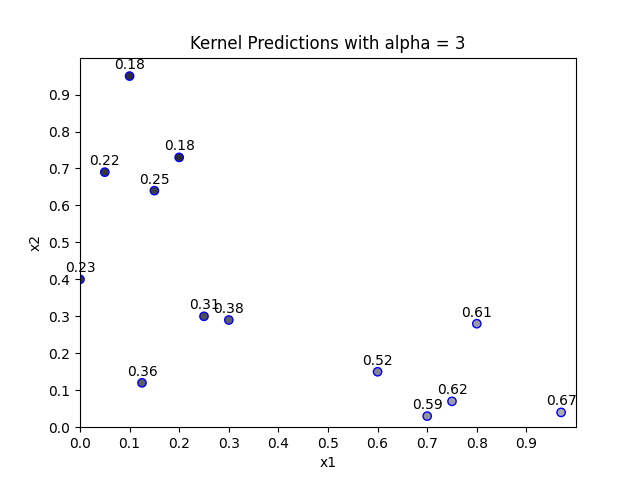
\includegraphics[scale=0.6]{alpha3.png}

    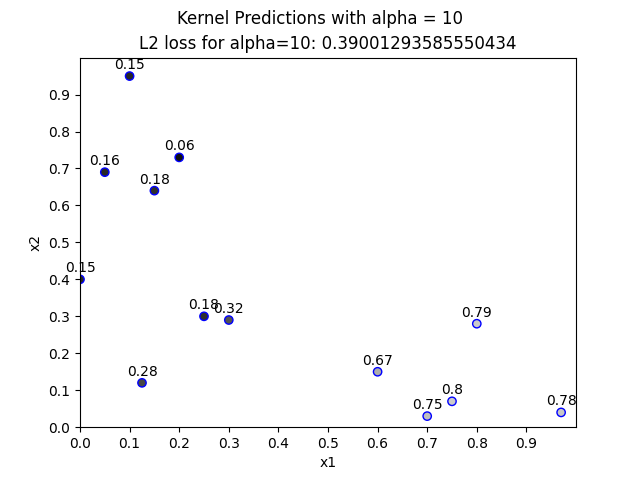
\includegraphics[scale=0.6]{alpha10.png}

    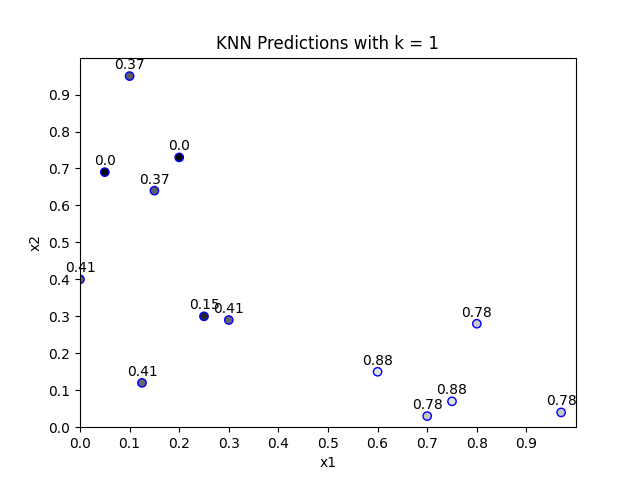
\includegraphics[scale=0.6]{k1.png}

    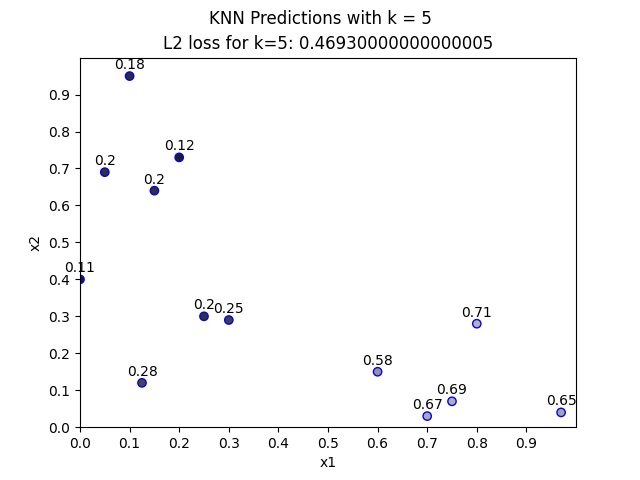
\includegraphics[scale=0.6]{k5.png}

    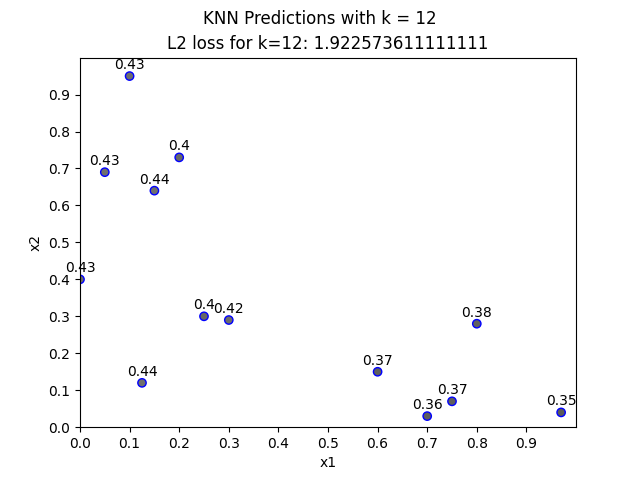
\includegraphics[scale=0.6]{k12.png}

    \item The choice of alpha is essentially a discount factor. The higher $\alpha$ is, the more we discount points by their distance from the input when we go to compute our distance metric (Mahalanobis here). To see this quantitatively with our example, note that a higher alpha will inflate the terms of $W$, leading us to compute $K$ where we are raising to a larger negative factor, which pushes the value of $K$ down. If we conversely use a lower alpha, the oppositve will occur. The relative ranking of the weights does not change, only their actual values.

    The kernel plot for $\alpha=0.1$ looks similar to the (N-1)NN plot, though not exactly the same. Also, the plot for $\alpha=10$ looks similar to the plot for the 1NN. Note that that doesn't mean these pairs of plots look exactly the same, since the kernel plot will be weighting all the values of the dataset and calculating a weighted average of the $y$'s based on this, while the nearest neighbor plots are just taking averages based on a subset of the $y$'s, the size of the subset being chosen by $k$.

    However, it intuitively makes sense that the kernel plot for $\alpha=0.1$ looks similar to the (N-1)NN plot because $\alpha=0.1$ means that we do not underweight far away points as much, making their weight closer to that of nearer points, which produces an effect similar to if we were to take the average over all the $y$'s, though not exactly the same. Similarly, it intuitively makes sense that the kernel plot for $\alpha=10$ looks similar to the 1NN plot because $\alpha=10$ means that we discount points that are farther away more (put even less weight on them than if $\alpha=1$), making these distant points' weights go closer to 0, which produces an effect similar to if we were to put most of the weight on the closest data point, similar to what a 1NN would do (``put all the weight on the closest point" and just use that data point's $y$ value as the predicted $\hat{y}$) but not exactly equal.

    \item We will show this is true by selecting a particular dataset and a particular $k$ and showing that for this dataset and this $k$, no value of alpha will produce kernel and kNN classifiers that make the same predictions.

    Consider a dataset of 3 points which are equidistant from each other on the $x_1, x_2$ plane (if we were to graph them on this plane, they would be arranged like the vertices of an equilateral triangle). Say the $y$ values for these datapoints is 0, 1, and 2, assigned arbitrarily. Consider what our prediction would be using a 1NN on the data point whose $y=2$. Your nearest neighbor is either the point with $y$ value of 1 or the point with $y$ value of 0. Your classifier would somehow break this tie and would have to choose either $y=1$ or $y=0$ to be the prediction for this input.

    From the perspective of kernel-based regression, since the two points are weighted equally, you would always get a prediction for this input that averages $y=1$ and $y=0$ to get 0.5. It would be impossible to get a prediction with a kernel-based regressor of 1 or 0 because that would imply that all of the weight is on one point or the other, which is impossible since the two data points are equidistant from the input and thus cannot have different weight.

    A similar argument can be made for each of the inputs in this dataset. Thus, by this example, for $k=1$, no value of $\alpha$ will produce two classifiers that are the same.

    \item We do not vary the $\alpha$ for the kNN because changing alpha does not change the relative ranking of the weights, only their actual values. Increasing alpha would stretch the relative rankings such that more distant points have their weights pushed to 0 more quickly and the opposite if we were to decrease alpha, as explained previously. However, this would not perturb the relative ranking of the Mahalanobis distances to each data point, which means that no matter how we vary alpha, we would still select the same $k$ nearest neighbors and take the average of their $y$'s. Thus, varying alpha would not change our outcome with the kNN approach, so we didn't vary it.
\end{enumerate}
\newpage

%%%%%%%%%%%%%%%%%%%%%%%%%%%%%%%%%%%%%%%%%%%%%
% Problem 3
%%%%%%%%%%%%%%%%%%%%%%%%%%%%%%%%%%%%%%%%%%%%%

\begin{problem}[Deriving Linear Regression, 10pts]

  In class, we noted that the solution for the least squares linear
  regressions ``looked'' like a ratio of covariance and variance
  terms.  In this problem, we will make that connection more explicit.

  Let us assume that our data are tuples of scalars $(x,y)$ that come from
  some distribution $p(x,y)$.  We will consider the process of fitting
  these data with the best linear model possible, that is a linear
  model of the form $\hat{y} = wx$ that minimizes the expected squared
  loss $E_{x,y}[ ( y - \hat{y} )^2 ]$.\\

\noindent \emph{Notes:} The notation $E_{x, y}$ indicates an
expectation taken over the joint distribution $p(x,y)$.  Since $x$ and
$y$ are scalars, $w$ is also a scalar.

  \begin{enumerate}

  \item Derive an expression for the optimal $w$, that is, the $w$
    that minimizes the expected squared loss above.  You should leave
    your answer in terms of moments of the data, e.g. terms like
    $E_x[x]$, $E_x[x^2]$, $E_y[y]$, $E_y[y^2]$, $E_{x,y}[xy]$ etc.

\item Provide unbiased and consistent formulas to estimate $E_{x, y}[yx]$
 and $E_x[x^2]$ given observed data $\{(x_n,y_n)\}_{n=1}^N$.

\item In general, moment terms like $E_{x, y}[yx]$, $E_{x, y}[x^2]$,
  etc. can easily be estimated from the data (like you did above).  If
  you substitute in these empirical moments, how does your expression
  for the optimal $w^*$ in this problem compare with the optimal $w^*$
  that we derived in class/Section 2.6 of the cs181-textbook?

\item As discussed in lecture, many common probabilistic linear regression models assume that variables x and y are jointly Gaussian.  Did any of your above derivations rely on the assumption that x and y are jointly Gaussian?  Why or why not?

\end{enumerate}

\end{problem}

\newpage

Problem 3 Solution:

\begin{enumerate}
    \item We can rewrite the expected squared loss as follows:

    $$E_{x, y}[(y-wx)^2] = \int_{x}\int_{y} (y-wx)^2p(x,y) dxdy$$

    The $w$ that minimizes this expression can be derived by setting the expression's derivative WRT $w$ equal to zero and solving for $w$:

    $$\pdv{}{w}\int_{x}\int_{y} (y-wx)^2p(x,y) dxdy = 0$$

    $$\int_{x}\int_{y} -2yxp(x,y) dxdy + \int_{x}\int_{y} 2wx^2p(x,y) dxdy=0$$

    $$w = \frac{\int_{x}\int_{y} yxp(x,y) dxdy}{\int_{x}\int_{y} x^2p(x,y) dxdy}$$

    $$w = \frac{E_{x, y}[xy]}{E_{x, y}[x^2]}$$

    We can also clearly see that the S.O.C WRT $w$ is equal to 1, meaning that our expected squared loss function is convex, meaning that our expression for $w$ is a minimum, as desired.

    \item With discrete dataset values, our expectations become summations rather than integrals. We see that $E_{x, y}[xy] = \sum_{n=1}^N \frac{x_ny_n}{N}$, since each pair $(x_n, y_n)$ (these pairs not necessarily distinct over all n) occurs in the dataset with probability $\frac{1}{N}$, by our observation. Similarly, $E_{x}[x^2] = \sum_{n=1}^N \frac{x^2_n}{N}$, since by our observation, each $x_n$ occurs in the dataset with probability $\frac{1}{N}$.

    \item If we substitute our empirical moments in, we get the following:

    $$w = \frac{E_{x, y}[xy]}{E_{x, y}[x^2]}$$

    $$w = \frac{\sum_{n=1}^N \frac{x_ny_n}{N}}{\sum_{n=1}^N \frac{x^2_n}{N}}$$

    $$w = \frac{\sum_{n=1}^N x_ny_n}{\sum_{n=1}^N x^2_n}$$

    $$w = \frac{\vec{x}^T\vec{y}}{\vec{x}^T\vec{x}}$$

    Above $\vec{x}$ denotes a column vector of all the individual $x_n$'s in our dataset, and similarly for $\vec{y}$.

    We can see that this is the same as the $w^*$ in the book, which was written as $W^* = (X^TX)^{-1}X^TY$, which is the same barring some slight notational differences. Thus, by substituting in empirical moments to minimize loss WRT a dataset, we can derive our expression for $w^*$ seen in the book, which assumed a dataset.

    \item No, our derivations did not rely on the assumption that $x$ and $y$ are jointly Gaussian, as we could be using any type of joint distribution $p(x,y)$ in the expressions. If $x$ and $y$ are indeed not jointly Gaussian though, we might notice patterns in the loss, high loss for select values, other signs, etc., that would signal to us that our assumption is not valid.
\end{enumerate}


%%%%%%%%%%%%%%%%%%%%%%%%%%%%%%%%%%%%%%%%%%%%%
% Problem 4
%%%%%%%%%%%%%%%%%%%%%%%%%%%%%%%%%%%%%%%%%%%%%

\begin{problem}[Modeling Changes in Republicans and Sunspots, 15pts]

 The objective of this problem is to learn about linear regression
 with basis functions by modeling the number of Republicans in the
 Senate. The file \verb|data/year-sunspots-republicans.csv| contains the
 data you will use for this problem.  It has three columns.  The first
 one is an integer that indicates the year.  The second is the number
 of Sunspots observed in that year.  The third is the number of Republicans in the Senate for that year.
 The data file looks like this:
 \begin{csv}
Year,Sunspot_Count,Republican_Count
1960,112.3,36
1962,37.6,34
1964,10.2,32
1966,47.0,36
\end{csv}

You can see scatterplots of the data in the figures below.  The horizontal axis is the Year, and the vertical axis is the Number of Republicans and the Number of Sunspots, respectively.

\begin{center}
\includegraphics[width=.5\textwidth]{data/year-republicans}
\end{center}

\begin{center}
\includegraphics[width=.5\textwidth]{data/year-sunspots}
\end{center}

(Data Source: \url{http://www.realclimate.org/data/senators_sunspots.txt})\\
\vspace{-5mm}


\vspace{0.5cm}
\noindent\emph{Make sure to include all required plots in your PDF.}

\begin{enumerate}

\item In this problem you will implement ordinary least squares regression using 4 different basis functions for
\textbf{Year (x-axis)} v. \textbf{Number of Republicans in the Senate (y-axis)}. Some starter Python code
that implements simple linear regression is provided in \verb|T1_P4.py|.

First, plot the data and regression lines for each of the following sets of basis functions, and include
the generated plot as an image in your submission PDF. You will therefore make 4 total plots:
\begin{enumerate}
	\item[(a)] $\phi_j(x) = x^j$ for $j=1, \ldots, 5$\\
    ie, use basis $y = a_1 x^1 + a_2 x^2 + a_3 x^3 + a_4 x^4 + a_5 x^5$ for some constants $\{a_1, ..., a_5\}$.
    \item[(b)] $\phi_j(x) = \exp{\frac{-(x-\mu_j)^2}{25}}$ for $\mu_j=1960, 1965, 1970, 1975, \ldots 2010$
	\item[(c)] $\phi_j(x) = \cos(x / j)$ for $j=1, \ldots, 5$
	\item[(d)] $\phi_j(x) = \cos(x / j)$ for $j=1, \ldots, 25$
\end{enumerate}
\vspace{-2mm}
{\footnotesize * Note: Be sure to add a bias term for each of the basis functions above.}

Second, for each plot include the residual sum of squares error. Submit the generated plot and residual sum-of-squares error for each basis in your LaTeX write-up.
\end{enumerate}

\end{problem}

\begin{framed}
\noindent\textbf{Problem 4} (cont.)\\
\begin{enumerate}
\setcounter{enumi}{1}
\item Repeat the same exact process as above but for \textbf{Number of Sunspots (x-axis)} v. \textbf{Number of Republicans in the Senate (y-axis)}.
Now, however, only use data from before 1985, and only use basis functions (a), (c), and (d) -- ignore basis (b). You will therefore make 3 total plots. For each plot make sure to also include the residual sum of squares error.

Which of the three bases (a, c, d) provided the "best" fit? \textbf{Choose one}, and keep in mind the generalizability of the model.

Given the quality of this fit, do you believe that the number of sunspots controls the number of Republicans in the senate (Yes or No)?
\end{enumerate}
\end{framed}

\newpage

Problem 4 Solution:

\begin{enumerate}
    \item My plots, with errors included as a subtitle and also printed to terminal:

    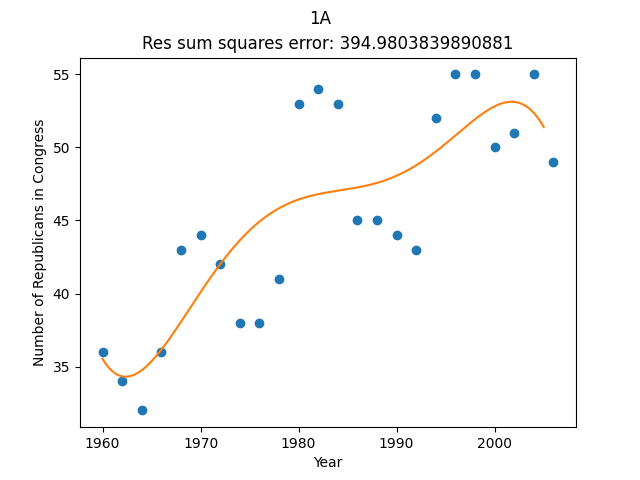
\includegraphics[scale=0.6]{plot-4-1a.png}

    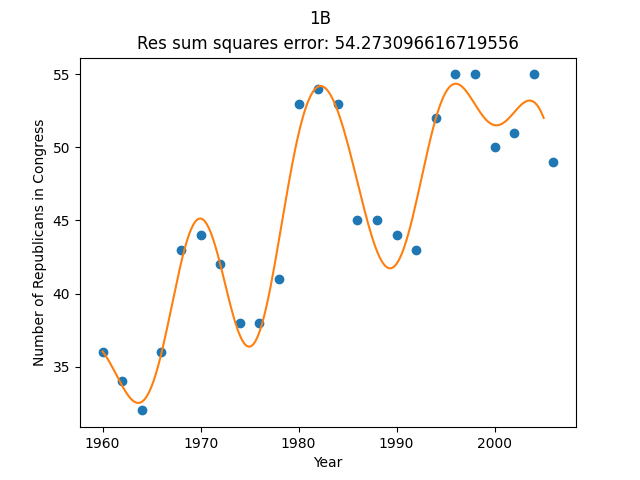
\includegraphics[scale=0.6]{plot-4-1b.png}

    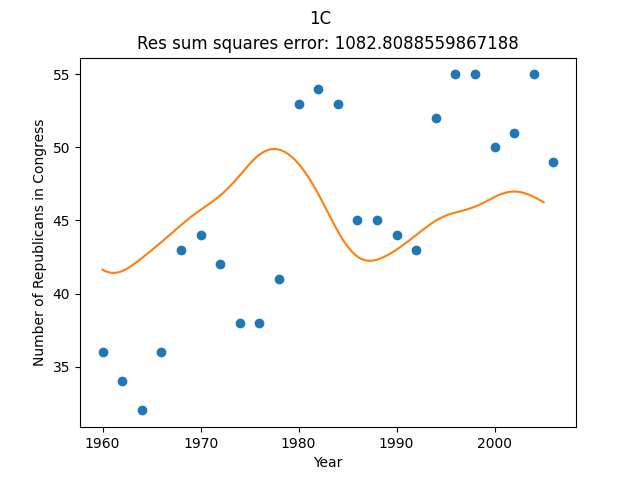
\includegraphics[scale=0.6]{plot-4-1c.png}

    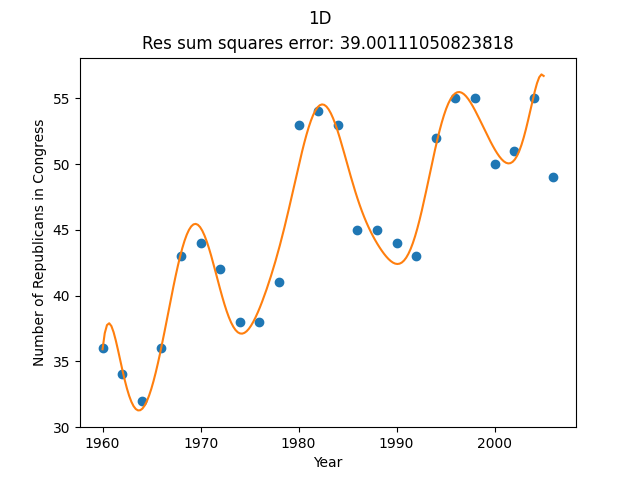
\includegraphics[scale=0.6]{plot-4-1d.png}

    \item My plots, with errors included as a subtitle and also printed to terminal:

    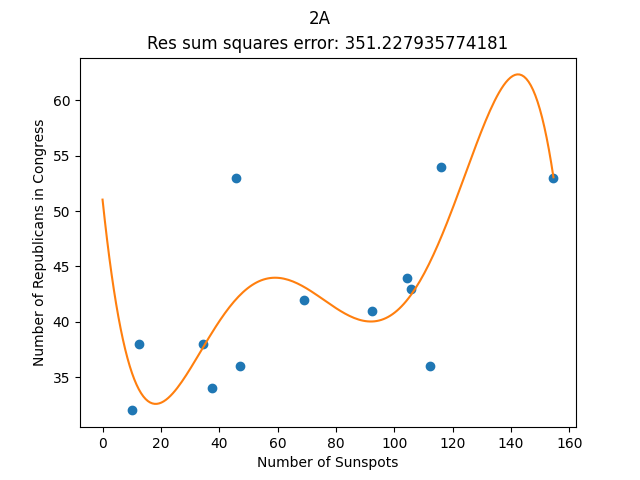
\includegraphics[scale=0.6]{plot-4-2a.png}

    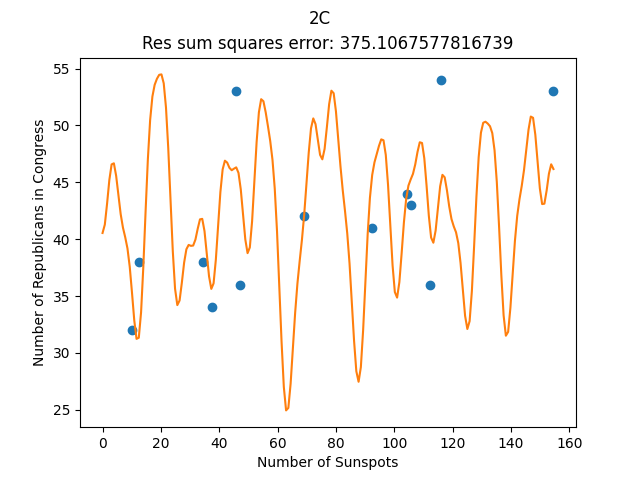
\includegraphics[scale=0.6]{plot-4-2c.png}

    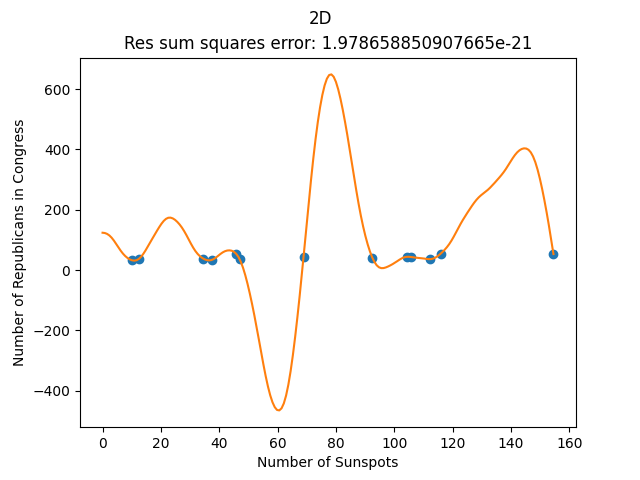
\includegraphics[scale=0.6]{plot-4-2d.png}

    I would say that basis (a) provided the "best" fit. Though this basis did not result in the lowest loss, the basis that did give the lowest loss (basis (d)), resulted in a wave pattern fit with very high "amplitude" in areas where we did not have much data, such as what the number of republicans has been when the number of sunspots has ranged from 20 to  around 35. This resulted in predictions where we might predict that when the number of sunspots is 60, there are around -400 Republicans in Congress, which is impossible. Thus, this curve might have fit our existing data to a very low loss, but is not generalizeable to more/other data on this relationship.

    Basis (c) gave a regression line that was very jagged, and whose first derivative tended to take more extreme values. We can imagine if the number of sunspots were to vary by a little over time, we would expect to see a possibly very large change in number of Republicans based on this model, which might not be generally true. This might lead to poor predictions in practice. This regression also had the highest loss. For all these reasons, this basis is not the best fit.

    In contrast, basis (a) does not exhibit these undesirable characteristics in the fit it gives, making its associated model the best and likely most generalizeable.

    Still what we have found here is a correlation between the two variables (number of sunspots and number of Republicans in Congress). Regression lines with strong fit, however we evaluate "fit", do not imply that one variable \textbf{causes}/controls the other variable. Regression can only help establish correlation between variables; if we want to know if one variable controls the other, we would need to perform an experimental study.
\end{enumerate}

\newpage
%%%%%%%%%%%%%%%%%%%%%%%%%%%%%%%%%%%%%%%%%%%%%
% Name and Calibration
%%%%%%%%%%%%%%%%%%%%%%%%%%%%%%%%%%%%%%%%%%%%%
\subsection*{Name}

Kathryn Wantlin

\subsection*{Collaborators and Resources}
Whom did you work with, and did you use any resources beyond cs181-textbook and your notes?

Office hours: Jonathan, Karthik, Andrew, Ife, Nari, and other attendees of this OH

\subsection*{Calibration}
Approximately how long did this homework take you to complete (in hours)?

12 hours
\end{document}
